\tikzset{
  invisible/.style={opacity=0},
  transparent/.style={opacity=0.2},
  visible on/.style={alt={#1{}{invisible}}},
  transparent on/.style={alt={#1{transparent}{}}},
  alt/.code args={<#1>#2#3}{%
    \alt<#1>{\pgfkeysalso{#2}}{\pgfkeysalso{#3}} % \pgfkeysalso doesn't change the path
  },
}

% Self arc
\def\centerarc[#1](#2)(#3:#4:#5)% Syntax: [draw options] (center) (initial angle:final angle:radius)
    { \draw[#1] ($(#2)+({#5*cos(#3)},{#5*sin(#3)})$) arc (#3:#4:#5); }

\begin{frame}{Time Series Pairwise Distance Calculation}
    \begin{figure}[t]
  \centering
    \begin{tikzpicture}
      \begin{axis}[%
        axis lines = none,
        height     =  8cm,
        width      =  11.0cm,
      ]
        \addplot[Set1-A, thick, no marks, visible on=<1-5>] table[x=x, y=a, col sep=comma] {./data/overview_TS_uneq_length_1.csv};
        \addplot[
          Set1-B, thick, no marks,
          y filter/.expression = {
            y - 10
          },
          visible on=<2>,
          transparent on=<3-5>
        ] table[x=x, y=a, col sep=comma] {./data/overview_TS_2.csv};
        
        \addplot[
          Set1-B, thick, no marks,
          x filter/.expression = {
            x + 130
          },
          y filter/.expression = {
            y - 10
          },
          visible on=<3>,
          transparent on=<4-5>
        ] table[x=x, y=a, col sep=comma] {./data/overview_TS_3.csv};
        \addplot[
          Set1-B, thick, no marks,
          x filter/.expression = {
            x + 260
          },
          y filter/.expression = {
            y - 10
          },
          visible on=<4>,
          transparent on=<5-5>
        ] table[x=x, y=a, col sep=comma] {./data/overview_TS_3.csv};
        \addplot[
          Set1-B, thick, no marks,
          x filter/.expression = {
            x + 390
          },
          y filter/.expression = {
            y - 10
          },
          visible on=<5>,
        ] table[x=x, y=a, col sep=comma] {./data/overview_TS_2.csv};
        % TODO create new timeseries..
        
        \filldraw[fill=ETHa, draw=ETHa, fill opacity=0.0] (280,112) rectangle (320,128);
        \filldraw<2->[fill=ETHa, draw=ETHa, fill opacity=0.7] (320,112) rectangle (360,128);
        \filldraw<3->[fill=ETHa, draw=ETHa, fill opacity=0.6] (360,112) rectangle (400,128);
        \filldraw<4->[fill=ETHa, draw=ETHa, fill opacity=0.2] (400,112) rectangle (440,128);
        \filldraw<5->[fill=ETHa, draw=ETHa, fill opacity=0.8] (440,112) rectangle (480,128);
        
        \draw<2>[draw opacity=0.8, line width=1pt] (50.00,90.00) -- (50.00,40.);
        \node<1-5> at (200,120) {$\wasserstein_1\left(\oneseries_0, \oneseries_\only<1>{0}\only<2>{1}\only<3>{2}\only<4>{3}\only<5>{4}\right)$};
        \draw<3>[draw opacity=0.8, line width=1pt] (50.00,90.00) -- (180.00,40.);
        \draw<4>[draw opacity=0.8, line width=1pt] (50.00,90.00) -- (310.00,40.);
        \draw<5>[draw opacity=0.8, line width=1pt] (50.00,90.00) -- (440.00,40.);
        % \centerarc[black,thick](10,100)(30:270:10)
        
        % SECOND ROW
        \addplot[
          Set1-B, thick, no marks,
          y filter/.expression = {
            y - 1
          },
          visible on=<6->
        ] table[x=x, y=a, col sep=comma] {./data/overview_TS_2.csv};
        
        \addplot[
          Set1-A, thick, no marks,
          y filter/.expression = {
            y - 10
          },
          visible on=<6>,
          transparent on=<7->
        ] table[x=x, y=a, col sep=comma] {./data/overview_TS_uneq_length_1.csv};
        \addplot[ % Had to copy it twice
          Set1-B, thick, no marks,
          x filter/.expression = {
            x + 130
          },
          y filter/.expression = {
            y - 10
          },
          visible on=<8>,
        ] table[x=x, y=a, col sep=comma] {./data/overview_TS_3.csv};
        \filldraw<6->[fill=ETHa, draw=ETHa, fill opacity=0.7] (280,98) rectangle (320,112);
        \filldraw<7->[fill=ETHa, draw=ETHa, fill opacity=0.0] (320,98) rectangle (360,112);
        \filldraw<8->[fill=ETHa, draw=ETHa, fill opacity=0.4] (360,98) rectangle (400,112);
        
        % Complete the square for future references
        
        % \filldraw<9->[fill=ETHa, draw=ETHa, fill opacity=0.8] (400,98) rectangle (440,112);
        % \filldraw<9->[fill=ETHa, draw=ETHa, fill opacity=0.5] (440,98) rectangle (480,112);
        
        % \filldraw<9->[fill=ETHa, draw=ETHa, fill opacity=0.6] (280,82) rectangle (320,98);
        % \filldraw<9->[fill=ETHa, draw=ETHa, fill opacity=0.4] (320,82) rectangle (360,98);
        % \filldraw<9->[fill=ETHa, draw=ETHa, fill opacity=0.0] (360,82) rectangle (400,98);
        % \filldraw<9->[fill=ETHa, draw=ETHa, fill opacity=0.1] (400,82) rectangle (440,98);
        % \filldraw<9->[fill=ETHa, draw=ETHa, fill opacity=0.2] (440,82) rectangle (480,98);
        
        % \filldraw<9->[fill=ETHa, draw=ETHa, fill opacity=0.2] (280,66) rectangle (320,82);
        % \filldraw<9->[fill=ETHa, draw=ETHa, fill opacity=0.8] (320,66) rectangle (360,82);
        % \filldraw<9->[fill=ETHa, draw=ETHa, fill opacity=0.1] (360,66) rectangle (400,82);
        % \filldraw<9->[fill=ETHa, draw=ETHa, fill opacity=0.0] (400,66) rectangle (440,82);
        % \filldraw<9->[fill=ETHa, draw=ETHa, fill opacity=0.2] (440,66) rectangle (480,82);
        
        % \filldraw<9->[fill=ETHa, draw=ETHa, fill opacity=0.8] (280,50) rectangle (320,66);
        % \filldraw<9->[fill=ETHa, draw=ETHa, fill opacity=0.5] (320,50) rectangle (360,66);
        % \filldraw<9->[fill=ETHa, draw=ETHa, fill opacity=0.2] (360,50) rectangle (400,66);
        % \filldraw<9->[fill=ETHa, draw=ETHa, fill opacity=0.2] (400,50) rectangle (440,66);
        % \filldraw<9->[fill=ETHa, draw=ETHa, fill opacity=0.0] (440,50) rectangle (480,66);
        
        
        \draw<6>[draw opacity=0.8, line width=1pt] (50.00,70.00) -- (50.00,40.);
        \node at (200,106) {$\wasserstein_1\left(\oneseries_1, \oneseries_\only<6>{0}\only<7>{1}\only<8>{2}\right)$};
        \draw<8>[draw opacity=0.8, line width=1pt] (50.00,70.00) -- (180.00,40.);
        
        
      \end{axis}
    \end{tikzpicture}
  \end{figure}
\end{frame}


\begin{frame}{Wasserstein Distance Matrix}
    \centering
    \LARGE
    $\mathcal{D} = $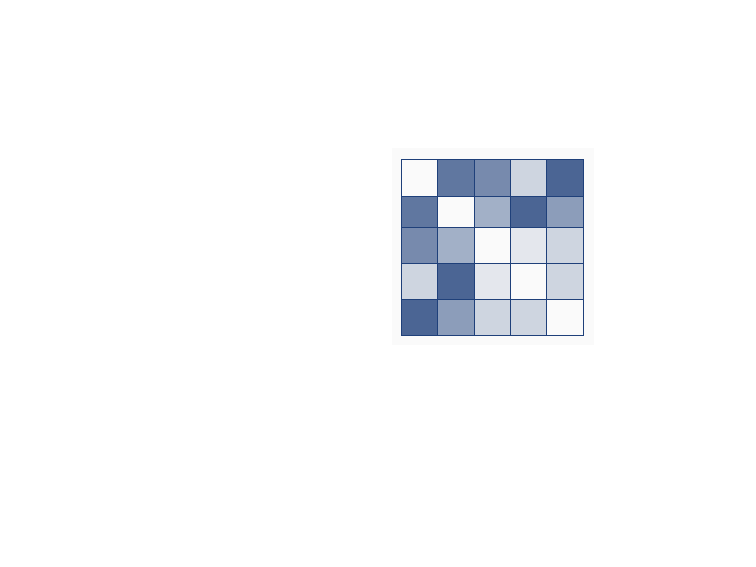
\includegraphics[width=0.5\textwidth,valign=c]{figures/distance_matrix.pdf} $\in \real^{|\allseries|\times |\allseries|}$ \\
    $\mathcal{D}_{ij} = \wasserstein_1\left(\oneseries_i, \oneseries_j\right)$
    
\end{frame}

\begin{frame}{From Distance to Kernels}
  \begin{definition}[Wasserstein time series kernel]
  \normalsize
  Let $\oneseries_i$ and $\oneseries_j$ be two time series, and $\shapelet_{i1}, \dots, \shapelet_{iU}$
  as well as $\shapelet_{j1}, \dots, \shapelet_{jV}$ be their respective
  subsequences. Moreover, let $D$ be a $U \times V$ matrix that contains
  the pairwise distances of all subsequences, such that
  %
  $D_{uv} := \dist\left(\shapelet_{iu}, \shapelet_{jv}\right)$,
  %
  where $\dist(\cdot, \cdot)$ denotes the usual Euclidean distance.
  The optimisation problem
  %
  \begin{equation}\
   \wasserstein_1\left(\oneseries_i, \oneseries_j\right) := \min_{P \in \Gamma\left(\oneseries_i, \oneseries_j\right)} \left\langle D, P \right\rangle_{\mathrm{F}},
    \label{eq:Our distance}
  \end{equation}
  %
  yields the optimal transport cost to transform $\oneseries_i$
  into $\oneseries_j$ by means of their subsequences. Then, given
  $\lambda\in\real_{> 0}$, we can define
  %
  \begin{equation}
    \Method\left(\oneseries_i, \oneseries_j\right) := \exp\left(-\lambda \wasserstein_1\left(\oneseries_i, \oneseries_j\right)\right),
    \label{eq:Our kernel}
  \end{equation}
  %
  which we refer to as our \emph{Wasserstein-based subsequence kernel};
  \end{definition}
\end{frame}

%%%%%%%%%%%%%%%%%%%%%%%%%%%%%%%%%%%%%%%%%%%%%%%%%%%%%%%%%%%%%%%%%%%%%%%%
% Algorithms
%%%%%%%%%%%%%%%%%%%%%%%%%%%%%%%%%%%%%%%%%%%%%%%%%%%%%%%%%%%%%%%%%%%%%%%%

\definecolor{mydarkblue}{rgb}{0,0.08,0.45}

\renewcommand{\algorithmicrequire}{\textbf{Input:}}
\renewcommand{\algorithmicensure}{\textbf{Output:}}
\renewcommand{\algorithmiccomment}[1]{\qquad \textcolor{ETHf}{//} \textcolor{ETHf}{#1}}

\begin{frame}{\longmethod}
    \begin{algorithm}[H]
      \footnotesize
      \caption{\longmethod}
      \begin{algorithmic}[1]
        \REQUIRE{Time series for training and testing
        $\allseries_{\text{train}}$, $\allseries_{\text{test}}$; subsequence
        length $w$; kernel weight factor $\lambda$}
        \ENSURE{$\mathcal{K}^{\,\text{train}}, \mathcal{K}^{\,\text{test}}$}
          \STATE $\shapelets^{\text{train}} \gets \textsc{Subsequences}({\allseries_{\text{train}}, w})$  \COMMENT{Extract subsequences}
          \STATE $\shapelets^{\text{test}} \gets \textsc{Subsequences}({\allseries_{\text{test}}, w})$ \COMMENT{Extract subsequences}
          \FOR{$\oneseries_i \in \allseries_{\text{train}}$}
            \FOR{$\oneseries_j \in \allseries_{\text{train}}$}
              \STATE $\mathcal{D}_{ij}^{\text{train}} \gets \wasserstein_1\left(\shapelets_i^{\text{train}}, \shapelets_j^{\text{train}}\right)$ \COMMENT{Wasserstein distance calculation (train)} %\Comment{Compute Wasserstein distance between TS using subsequences}
            \ENDFOR
          \FOR{$\oneseries_k \in \allseries_{\text{test}}$}
            \STATE $\mathcal{D}_{ik}^{\text{test}} \gets \wasserstein_1\left(\shapelets_i^{\text{train}}, \shapelets_k^{\text{test}}\right)$ \COMMENT{Wasserstein distance calculation (test)} %\Comment{Compute Wasserstein distance between TS using subsequences}
            \ENDFOR
          \ENDFOR
          \STATE $\mathcal{K}^{\,\text{train}} \gets \exp\left(-\lambda \mathcal{D}^{\text{train}} \right)$ \COMMENT{Kernel matrix calculation}
          \STATE $\mathcal{K}^{\,\text{test}} \gets \exp\left(-\lambda \mathcal{D}^{\text{test}} \right)$ \COMMENT{Kernel matrix calculation}
          \RETURN $\mathcal{K}^{\,\text{train}}, \mathcal{K}^{\,\text{test}}$
      \end{algorithmic}
    \end{algorithm}
\end{frame}